\documentclass[11pt]{amsart}

\usepackage[margin=1in]{geometry}
\usepackage[T1]{fontenc}
\usepackage{amsmath,amssymb,amsthm,url,enumitem,booktabs,tabularx,array}
\usepackage{xcolor}
\usepackage{tikz}
\usetikzlibrary{arrows.meta}

\newtheorem{theorem}{Theorem}
\newtheorem{corollary}[theorem]{Corollary}
\newtheorem{lemma}[theorem]{Lemma}
\newtheorem{proposition}[theorem]{Proposition}
\newtheorem{remark}[theorem]{Remark}

\newcommand{\N}{\mathbb{N}}

\title{Forbidden subgraphs in divisor graphs and an Erd\H{o}s divisibility problem}
\author{Damek Davis}
\thanks{Research supported by NSF DMS award 2523384.}
\address{Department of Statistics and Data Science, The Wharton School, University of Pennsylvania}
\email{damek@wharton.upenn.edu}
\date{}

\begin{document}

\begin{abstract}
Erd\H{o}s asked for the largest size $f(n)$ of a subset of $\{1,\dots,n\}$ with no element dividing two others, and whether $\lim f(n)/n$ is irrational. We show that $f(n)=c_2\,n+o(n)$ for an effectively computable constant~$c_2$, and moreover that the number $q(n)$ of such subsets satisfies $q(n)=\beta_2^{n+o(n)}$ for a computable constant~$\beta_2$. More generally, we prove that any family of subsets of $\{1,\dots,n\}$ that is downward closed, decomposes over coprime components of the divisor graph, and is preserved by integer dilation has maximum size $c\,n+o(n)$ and count $\beta^{n+o(n)}$ for effectively computable constants $c$ and $\beta$. This covers forbidden connected subgraphs of the divisor graph and, more broadly, sets avoiding prescribed multiplicative ratio patterns, including the family of all $k$-term geometric progressions of integer ratio. The proof uses a theorem of McNew on local statistics of divisor graphs. The irrationality of~$c_2$ remains open.
\end{abstract}

\maketitle

\section{Introduction}

Let \(f(n)\) denote the largest size of a set \(A\subseteq \{1,\dots,n\}\) such that there do not exist distinct \(a,b,c\in A\) with \(a\mid b\) and \(a\mid c\). A question of Erd\H{o}s (see Guy~\cite[Problem~B24]{Gu04} and Bloom~\cite[Problem 1062]{BloomEP}) asks how large \(f(n)\) can be and whether \(\lim_{n\to\infty} f(n)/n\) is irrational. The interval \(\{\lfloor n/3\rfloor+1,\dots,n\}\) already shows that \(f(n)\ge \lceil 2n/3\rceil\). Lebensold~\cite{Le76} proved that for sufficiently large \(n\),
\[
0.6725\,n\le f(n)\le 0.6736\,n,
\]
and OEIS~A038372 tabulates the exact extremal values for small \(n\)~\cite{OEISA038372}.

In this note we prove that for every \(\varepsilon > 0\),
\[
f(n)=c_2\,n+O_{\varepsilon}\!\left(n\exp\!\bigl(-(1-\varepsilon)\sqrt{\log n\,\log\log n}\bigr)\right)
\]
for an effectively computable constant \(c_2\), and the number of such subsets has exponential growth rate~\(\beta_2\) for a computable constant~\(\beta_2\ge 1\) (Corollary~\ref{cor:erdos}). The key is to recast the problem in the \emph{divisor graph} on \(\{1,\dots,n\}\), whose vertices are joined whenever one divides the other; divisibility gives each edge a natural orientation from divisor to multiple, written \(u\to v\) when \(u\mid v\). The Erd\H{o}s condition---no element divides two others---is then equivalent to forbidding the directed \emph{two-fork} \(x\to y\), \(x\to z\). This makes the problem an instance of a \emph{vertex Tur\'an-type problem}: given a host graph~\(H\) and a forbidden subgraph~\(F\), find the largest vertex subset \(U\subseteq V(H)\) whose induced subgraph contains no copy of~\(F\). (The classical theorem of Tur\'an~\cite{Tu41} is the edge-maximization analogue.)

Our main result (Theorem~\ref{thm:general}) applies to any family of subsets of \(\{1,\dots,n\}\) satisfying three structural axioms---downward closed, componentwise over the divisor graph, and dilation-invariant---and gives both an extremal density \(c\,n+o(n)\) and an exponential counting rate~\(\beta^{n+o(n)}\). We derive two families of applications. The first (Corollary~\ref{cor:patterns}) concerns forbidden connected subgraphs of the divisor graph: for any finite family of such subgraphs, directed or undirected, the density and counting rate exist. The Erd\H{o}s two-fork is one instance (Corollary~\ref{cor:erdos}); further applications to \(r\)-fork avoidance and \(k\)-chain avoidance are given in Remark~\ref{par:applications}. For the Erd\H{o}s problem the orientation is essential, since the undirected two-fork would also forbid the reverse pattern---no element is a common multiple of two others---which is a different condition.

The second family of applications (Corollary~\ref{cor:ratio}) concerns sets avoiding prescribed multiplicative ratio patterns: given a collection~\(\mathcal{D}\) of finite sets of integers, each with \(\gcd(D)=1\) and connected divisor graph, the family of subsets of \(\{1,\dots,n\}\) containing no pattern \(\{d_1 m,\dots,d_k m\}\) for \(D\in\mathcal{D}\) satisfies the three axioms. When the prime support of~\(\mathcal{D}\) is finite, the density was computed by Graham, Spencer, and Witsenhausen~\cite{GSW77} (without requiring connectivity or a gcd condition); the corollary is most useful when the prime support is infinite, for instance establishing that \(\lim f_{\mathcal{D}}(n)/n\) exists when \(\mathcal{D}\) is the family of all \(k\)-term geometric progressions of integer ratio, for every \(k\ge 3\).

The main tool is a theorem of McNew~\cite{McNew21} on local statistics of divisor graphs, which expresses certain additive and multiplicative divisor-graph statistics as explicit convergent series. Theorem~\ref{thm:general} identifies a broad class of properties---those that are downward closed, decompose over coprime components, and are preserved by integer dilation---for which we use McNew's theorem to obtain both computable density and counting estimates. For the Erd\H{o}s two-fork case, the numerical estimates in Section~\ref{sec:numerical} improve Lebensold's lower bound to \(c_2\ge 0.672965\ldots\), narrowing the gap with his upper bound \(c_2\le 0.6736\) to about \(6.4\times 10^{-4}\), and give \(1.7294\ldots \le \beta_2 \le 1.8746\ldots\). Remark~\ref{par:applications} records further representative constants for other forbidden subgraphs.

McNew~\cite{McNew21} also uses his theorem to study other problems on the divisor graph. The most-studied case is the two-chain \(a\mid b\): sets avoiding it are called \emph{primitive}, and their extremal density is \(1/2\). Determining the counting rate is more involved: Angelo~\cite{Angelo18} proved that the number of primitive subsets of \(\{1,\dots,n\}\) has an exponential growth rate, and McNew~\cite[Theorem~2]{McNew21} obtained this rate with an explicit error term.

\section{Main results}\label{sec:general}

This section states the general theorem (Theorem~\ref{thm:general}), which gives both an extremal density and a counting result, derives its forbidden-subgraph corollary (Corollary~\ref{cor:patterns}), and specializes to the Erd\H{o}s problem (Corollary~\ref{cor:erdos}). We begin with the notation needed for the constants that appear in these results.

For any family \(\mathcal{P}\) of finite subsets of \(\N\) and any finite set \(T\subset\N\), write
\[
\Phi_{\mathcal{P}}(T):=\max\{|B|:B\subseteq T,\;B\in\mathcal{P}\},
\qquad
Q_{\mathcal{P}}(T):=\#\{B\subseteq T:B\in\mathcal{P}\}.
\]
Let \(P^+(d)\) denote the largest prime factor of \(d\), with \(P^+(1)=1\). For any function \(\Psi\) defined on finite subsets of \(\N\) for which the following series converges absolutely, define
\[
C_{\Psi}:=
\sum_{i=1}^{\infty}
\left(\prod_{p\le i}\frac{p-1}{p}\right)
\sum_{\substack{d\ge 1\\ P^+(d)\le i}}
\sum_{t\in[id,(i+1)d)}
\frac{\Psi(\{d,\dots,t\})-\Psi(\{d+1,\dots,t\})}{t(t+1)}.
\]
The coefficient weights in this series sum to~\(1\) (as we later see in~\eqref{eq:weight}), so \(C_\Psi\) converges absolutely whenever the differences \(\Psi(\{d,\dots,t\})-\Psi(\{d+1,\dots,t\})\) are uniformly bounded. In particular, \(C_{\Phi_{\mathcal{P}}}\) and \(C_{\log Q_{\mathcal{P}}}\) are well-defined for any family \(\mathcal{P}\) satisfying the hypotheses of the theorem below.

\begin{theorem}\label{thm:general}
Let \(\mathcal{P}\) be a family of finite subsets of \(\N\), called admissible sets, and assume \(\emptyset\in\mathcal{P}\). Assume further:
\begin{enumerate}
\item (downward closed) if \(B\in \mathcal{P}\) and \(B'\subseteq B\), then \(B'\in \mathcal{P}\);
\item (decomposes over coprime components) if \(T=T_1\sqcup T_2\) is finite and there is no divisibility relation between an element of \(T_1\) and an element of \(T_2\), then for every \(B\subseteq T\) we have \(B\in \mathcal{P}\) if and only if \(B\cap T_i\in \mathcal{P}\) for \(i=1,2\);
\item (preserved by integer dilation) if \(m\in \N\) and \(B\) is finite, then \(B\in \mathcal{P}\) if and only if \(mB\in \mathcal{P}\), where \(mB:=\{mb:\ b\in B\}\).
\end{enumerate}
Write \(f_{\mathcal{P}}(n):=\Phi_{\mathcal{P}}(\{1,\dots,n\})\), \(q_{\mathcal{P}}(n):=Q_{\mathcal{P}}(\{1,\dots,n\})\), \(c_{\mathcal{P}}:=C_{\Phi_{\mathcal{P}}}\), and \(\beta_{\mathcal{P}}:=\exp(C_{\log Q_{\mathcal{P}}})\).
Then for every \(\varepsilon>0\):
\begin{enumerate}[label=\textup{(\alph*)}]
\item \textup{(Extremal density.)}
\[
f_{\mathcal{P}}(n)=c_{\mathcal{P}}\,n+O_{\varepsilon}\!\left(
n\exp\!\bigl(-(1-\varepsilon)\sqrt{\log n\,\log\log n}\bigr)
\right).
\]

\item \textup{(Counting.)}
\[
\log q_{\mathcal{P}}(n)=n\log\beta_{\mathcal{P}}+O_{\varepsilon}\!\left(
n\exp\!\bigl(-(1-\varepsilon)\sqrt{\log n\,\log\log n}\bigr)
\right).
\]
In particular, \(\lim_{n\to\infty}q_{\mathcal{P}}(n)^{1/n}=\beta_{\mathcal{P}}\).
\end{enumerate}
If in addition membership in \(\mathcal{P}\) is decidable for finite sets, then \(c_{\mathcal{P}}\) and \(\beta_{\mathcal{P}}\) are effectively computable.
\end{theorem}

\noindent\textbf{Convention.} Throughout the paper we apply Theorem~\ref{thm:general} to various families~\(\mathcal{P}\) and denote the resulting constants by \(c_{\mathcal{P}}\), \(\beta_{\mathcal{P}}\), etc. In every application below, membership in~\(\mathcal{P}\) is decidable (often trivially so), and hence all such constants are effectively computable; we will not repeat this observation each time.

\begin{remark}[Partition function]\label{rem:partition}\rm
The same argument shows that for any fixed \(z>0\), the partition function \(Z_{\mathcal{P}}(T,z):=\sum_{B\subseteq T,\,B\in\mathcal{P}} z^{|B|}\) satisfies
\[
\log Z_{\mathcal{P}}(\{1,\dots,n\},z)
=\kappa_{\mathcal{P}}(\log z)\,n
+O_{\varepsilon}\!\left(
\log(1+z)\,n\exp\!\bigl(-(1-\varepsilon)\sqrt{\log n\,\log\log n}\bigr)
\right)
\]
for an effectively computable constant \(\kappa_{\mathcal{P}}(\log z)\). The case \(z=1\) is part~(b) of the theorem. It is straightforward to show that the ``pressure" \(t\mapsto\kappa_{\mathcal{P}}(t)\) is convex and \(1\)-Lipschitz, and \(\kappa_{\mathcal{P}}(t)/t\to c_{\mathcal{P}}\) as \(t\to\infty\).
\end{remark}

We now describe the family of admissible sets to which we apply Theorem~\ref{thm:general}. The \emph{divisor graph} of a finite set \(S\subset\N\) has vertex set \(S\) with an edge between \(u\) and \(v\) whenever \(u\ne v\) and one divides the other; we orient each edge from divisor to multiple, writing \(u\to v\) when \(u\mid v\). Given a collection \(\mathcal{F}\) of connected graphs, each directed or undirected---here connected refers to the underlying undirected graph, regardless of orientation---say that a finite set \(S\) is \emph{\(\mathcal{F}\)-free} if its divisor graph contains no copy of any member of~\(\mathcal{F}\): containment of a directed member means containment as a directed subgraph of the oriented divisor graph, while containment of an undirected member means containment as a subgraph of the underlying undirected graph. Write \(\mathcal{P}(\mathcal{F})\) for the family of all \(\mathcal{F}\)-free sets. We do not require the copy to be induced, so extra divisibility arrows among the chosen vertices are allowed.\footnote{If one instead requires induced containment, the three axioms still hold and Theorem~\ref{thm:general} applies equally. Non-induced avoidance is more restrictive and is the natural choice for the Erd\H{o}s problem, since ``no element divides two others'' does not depend on the relationship between those two others.} For example, \(\{1,2,4\}\) contains the two-fork \(x\to y\), \(x\to z\): the arrows \(1\to 2\) and \(1\to 4\) realize it, while the extra arrow \(2\to 4\) is harmless. Figure~\ref{fig:noninduced} illustrates this distinction, and Figure~\ref{fig:patterns} shows four representative connected forbidden subgraphs. The family \(\mathcal{P}(\mathcal{F})\) satisfies the three axioms of Theorem~\ref{thm:general}, giving the following corollary.

\begin{figure}[t]
\centering
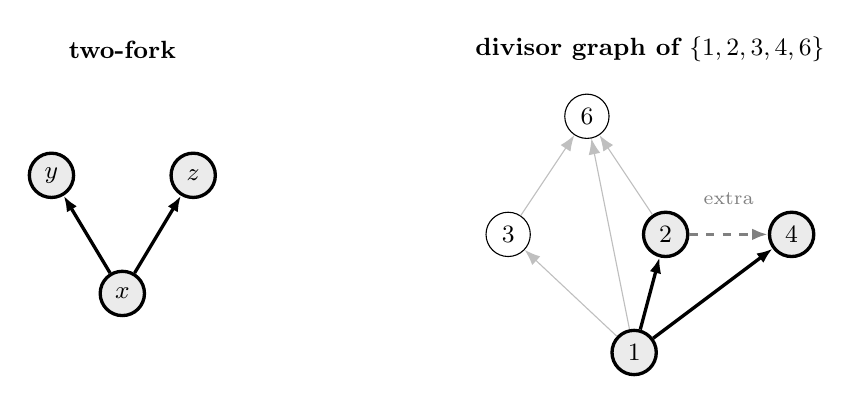
\begin{tikzpicture}[
    vertex/.style={circle,draw,inner sep=1.2pt,minimum size=16pt,font=\small},
    matched/.style={circle,draw,line width=1.2pt,fill=black!8,inner sep=1.2pt,minimum size=16pt,font=\small},
    bg/.style={-{Latex[length=2mm]},thin,black!25},
    pat/.style={-{Latex[length=2mm]},line width=1.2pt},
    extra/.style={-{Latex[length=2mm]},line width=1.2pt,dashed,black!50}
]
%%% Left: two-fork pattern (vertically centered with right graph)
\node[font=\small\bfseries] at (-2.5,3.85) {two-fork};
\begin{scope}[shift={(-2.5,0.75)}]
\node[matched] (px) at (0,0) {$x$};
\node[matched] (py) at (-0.9,1.5) {$y$};
\node[matched] (pz) at (0.9,1.5) {$z$};
\draw[pat] (px) -- (py);
\draw[pat] (px) -- (pz);
\end{scope}

%%% Right: divisor graph of {1,2,3,4,6}
\begin{scope}[shift={(4.0,0)}]
\node[font=\small\bfseries] at (0.2,3.85) {divisor graph of $\{1,2,3,4,6\}$};
% level 0: root
\node[matched] (v1) at (0,0) {$1$};
% level 1: primes/prime-powers
\node[vertex]  (v3) at (-1.6,1.5) {$3$};
\node[matched] (v2) at (0.4,1.5) {$2$};
\node[matched] (v4) at (2.0,1.5) {$4$};
% level 2: composite — centered between its divisors 2 and 3
\node[vertex]  (v6) at (-0.6,3.0) {$6$};
% background divisibility arrows (faded)
\draw[bg] (v1) -- (v3);
\draw[bg] (v1) -- (v6);
\draw[bg] (v3) -- (v6);
\draw[bg] (v2) -- (v6);
% pattern-matching arrows (bold): 1->2 and 1->4
\draw[pat] (v1) -- (v2);
\draw[pat] (v1) -- (v4);
% extra divisibility among matched vertices (dashed): 2|4
\draw[extra] (v2) -- (v4);
\node[font=\scriptsize,black!50] at (1.2,1.95) {extra};
\end{scope}
\end{tikzpicture}
\caption{Non-induced subgraph containment. \textbf{Left:} the two-fork. \textbf{Right:} the divisor graph of $\{1,2,3,4,6\}$; the shaded vertices $\{1,2,4\}$ realize the two-fork via the bold arrows $1\to 2$ and $1\to 4$. The dashed arrow $2\to 4$ is an extra divisibility among the matched vertices; the copy need not be induced.}
\label{fig:noninduced}
\end{figure}

\begin{figure}[t]
\centering
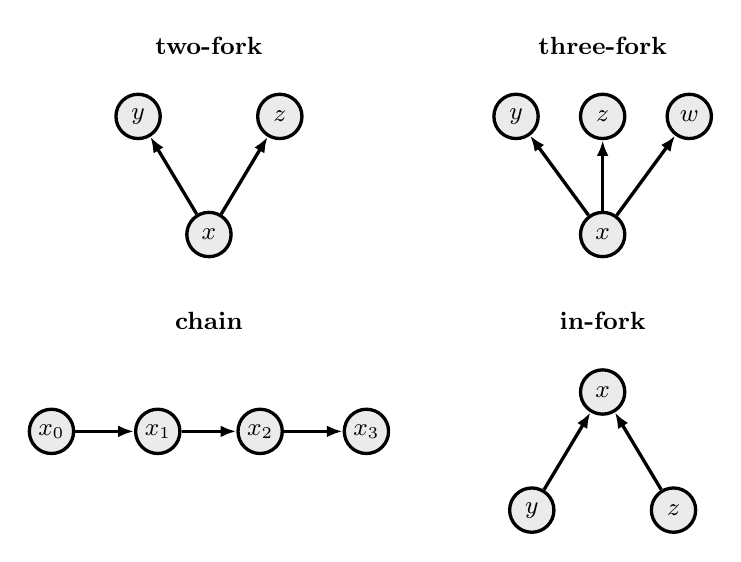
\begin{tikzpicture}[
    nd/.style={circle,draw,line width=1.2pt,fill=black!8,inner sep=1.2pt,minimum size=16pt,font=\small},
    arr/.style={-{Latex[length=2mm]},line width=1.2pt}
]
% two-fork
\begin{scope}[shift={(0,0)}]
\node[font=\small\bfseries] at (0,2.4) {two-fork};
\node[nd] (a1) at (0,0) {$x$};
\node[nd] (b1) at (-0.9,1.5) {$y$};
\node[nd] (c1) at (0.9,1.5) {$z$};
\draw[arr] (a1) -- (b1);
\draw[arr] (a1) -- (c1);
\end{scope}

% three-fork
\begin{scope}[shift={(5,0)}]
\node[font=\small\bfseries] at (0,2.4) {three-fork};
\node[nd] (a2) at (0,0) {$x$};
\node[nd] (b2) at (-1.1,1.5) {$y$};
\node[nd] (c2) at (0,1.5) {$z$};
\node[nd] (d2) at (1.1,1.5) {$w$};
\draw[arr] (a2) -- (b2);
\draw[arr] (a2) -- (c2);
\draw[arr] (a2) -- (d2);
\end{scope}

% chain
\begin{scope}[shift={(0,-3.5)}]
\node[font=\small\bfseries] at (0,2.4) {chain};
\node[nd] (a3) at (-2.0,1.0) {$x_0$};
\node[nd] (b3) at (-0.65,1.0) {$x_1$};
\node[nd] (c3) at (0.65,1.0) {$x_2$};
\node[nd] (d3) at (2.0,1.0) {$x_3$};
\draw[arr] (a3) -- (b3);
\draw[arr] (b3) -- (c3);
\draw[arr] (c3) -- (d3);
\end{scope}

% in-fork
\begin{scope}[shift={(5,-3.5)}]
\node[font=\small\bfseries] at (0,2.4) {in-fork};
\node[nd] (a4) at (0,1.5) {$x$};
\node[nd] (b4) at (-0.9,0) {$y$};
\node[nd] (c4) at (0.9,0) {$z$};
\draw[arr] (b4) -- (a4);
\draw[arr] (c4) -- (a4);
\end{scope}
\end{tikzpicture}
\caption{Representative connected forbidden subgraphs of divisor graphs. Arrows point from divisor to multiple.}
\label{fig:patterns}
\end{figure}


\begin{corollary}\label{cor:patterns}
Let \(\mathcal{F}\) be a finite family of connected\footnote{Connectedness is essential: a disconnected forbidden subgraph can straddle two connected components of the divisor graph, so the componentwise axiom may fail.} forbidden subgraphs (directed or undirected) of divisor graphs, and let \(f_{\mathcal{F}}(n)\) and \(q_{\mathcal{F}}(n)\) denote the maximum size, and the number, of \(\mathcal{F}\)-free subsets of \(\{1,\dots,n\}\). Applying Theorem~\ref{thm:general} to \(\mathcal{P}(\mathcal{F})\), there exist constants \(c_{\mathcal{F}}\) and \(\beta_{\mathcal{F}}\ge 1\) such that, for every \(\varepsilon>0\),
\begin{align*}
f_{\mathcal{F}}(n)&=c_{\mathcal{F}}\,n+O_{\varepsilon}\!\bigl(n\exp\!\bigl(-(1-\varepsilon)\sqrt{\log n\,\log\log n}\bigr)\bigr),\\
\log q_{\mathcal{F}}(n)&=n\log\beta_{\mathcal{F}}+O_{\varepsilon}\!\bigl(n\exp\!\bigl(-(1-\varepsilon)\sqrt{\log n\,\log\log n}\bigr)\bigr).
\end{align*}
\end{corollary}

\begin{proof}
Downward closure is immediate: passing to a subset cannot create a forbidden subgraph. For scale invariance, multiplication by any positive integer preserves divisibility, so \(B\) contains a forbidden subgraph if and only if \(mB\) does. For the componentwise axiom, let \(T=T_1\sqcup T_2\) with no divisibility between \(T_1\) and~\(T_2\). Any copy of a connected forbidden subgraph in~\(T\) is connected in the undirected divisor graph and therefore lies entirely in one~\(T_\ell\).
\end{proof}

Corollary~\ref{cor:patterns} is not the only source of examples for Theorem~\ref{thm:general}. The collection \(\mathcal{F}\) may also be infinite, or may mix directed and undirected patterns; the only additional requirement is that membership in \(\mathcal{P}(\mathcal{F})\) be decidable for finite sets (which is automatic when \(\mathcal{F}\) is finite). For instance, requiring the divisor graph of the chosen subset to be a forest---equivalently, forbidding all cycles as undirected subgraphs---satisfies the three axioms, so Theorem~\ref{thm:general} applies. This is a genuinely infinite family of forbidden subgraphs: for every \(k\ge 3\), taking \(k\)~distinct primes \(p_1,\dots,p_k\) and the products \(p_1 p_2,\, p_2 p_3,\,\dots,\, p_k p_1\) yields a set of~\(2k\) integers whose divisor graph is exactly~\(C_{2k}\) with no shorter cycle, so no finite subfamily suffices. More generally, for any fixed \(t\ge 1\), requiring the divisor graph to have treewidth at most~\(t\) satisfies the three axioms: treewidth is monotone under taking subgraphs, equals the maximum over connected components, and is preserved by dilation.

Specializing the corollary to the two-fork \(x\mid y\), \(x\mid z\) recovers the Erd\H{o}s problem:

\begin{corollary}\label{cor:erdos}
Let \(f(n)\) and \(q(n)\) denote the maximum size, and the number, of subsets of \(\{1,\dots,n\}\) containing no distinct \(x,y,z\) with \(x\mid y\) and \(x\mid z\). Then there exist constants \(c_2\) and \(\beta_2\ge 1\) such that, for every \(\varepsilon>0\),
\begin{align*}
f(n)&=c_2\,n+O_{\varepsilon}\!\left(n\exp\!\bigl(-(1-\varepsilon)\sqrt{\log n\,\log\log n}\bigr)\right),\\
\log q(n)&=n\log\beta_2+O_{\varepsilon}\!\left(n\exp\!\bigl(-(1-\varepsilon)\sqrt{\log n\,\log\log n}\bigr)\right).
\end{align*}
In particular, \(\lim_{n\to\infty}q(n)^{1/n}=\beta_2\).
\end{corollary}

The question of whether \(c_2\) is irrational, raised by Erd\H{o}s (see~\cite[Problem~B24]{Gu04}), remains open.

\begin{remark}[Forks, in-forks, and chains]\label{par:applications}\rm
Corollary~\ref{cor:patterns} applies equally to other connected forbidden subgraphs. For each \(r\ge 2\), the \(r\)-fork---forbidding any element from dividing \(r\) others---is connected, so the corollary gives computable density \(c_r\) and counting rate. The interval \((\lfloor n/(r+1)\rfloor,n]\) gives \(c_r\ge r/(r+1)\) and, since all of its subsets are admissible, \(\beta_r\ge 2^{r/(r+1)}\). For \(r\ge 3\), earlier bounds on \(c_r\) were obtained by Vijay~\cite{Vijay06} and Hegarty~\cite{Hegarty06}. Using the series representation of Section~\ref{sec:numerical} with a similar truncation, we estimate \(c_3\in[0.7523,\,0.8460]\) and \(\beta_3\in[1.7925,\,1.9490]\).

For each \(k\ge 2\), the directed path \(x_1\to x_2\to\cdots\to x_k\) on \(k\)~vertices is connected, so the corollary gives a computable density \(\gamma_k\) and counting rate \(\delta_k\) for \(k\)-chain-free subsets of \(\{1,\dots,n\}\). The interval \((\lfloor n/2^{k-1}\rfloor,n]\) is \(k\)-chain-free, giving \(\gamma_k\ge 1-2^{1-k}\) and \(\delta_k\ge 2^{1-2^{1-k}}\). For \(k=2\), \(\gamma_2=1/2\): a \(2\)-chain-free set is an antichain, and the \(\lceil n/2\rceil\) chains \(\{q,2q,4q,\dots\}\cap[1,n]\) for odd \(q\le n\) show this is tight.

Dually, the \(r\)-in-fork \(y_1\to x,\,\dots,\,y_r\to x\) forbids any element from being a multiple of \(r\) others. This is the problem dual to the \(r\)-fork, also posed by Erd\H{o}s~\cite[Problem~B24]{Gu04}. The in-fork is connected and directed, so Corollary~\ref{cor:patterns} gives a computable density \(c_r^*\) and counting rate for each \(r\ge 2\). The same interval \((\lfloor n/(r+1)\rfloor,n]\) is also \(r\)-in-fork-free, giving \(c_r^*\ge r/(r+1)\). Again using the series truncation of Section~\ref{sec:numerical}, one can estimate that \(c_2^*\in[0.7195,\,0.8340]\) and \(\beta_2^*\in[1.7550,\,1.9370]\), confirming that the in-fork and two-fork problems have different extremal densities.
\end{remark}

Theorem~\ref{thm:general} also applies to patterns defined by fixed multiplicative ratios, beyond the forbidden-subgraph framework of Corollary~\ref{cor:patterns}. Let \(\mathcal{D}\) be a collection (finite or infinite) of finite sets of distinct positive integers, each satisfying \(\gcd(D)=1\) and having connected divisor graph---that is, for every \(D=\{d_1,\dots,d_k\}\in\mathcal{D}\), the elements of~\(D\) have no common factor and can be linked by a chain of divisibility relations among themselves. Say that \(S\subseteq\{1,\dots,n\}\) is \emph{\(\mathcal{D}\)-free} if it contains no subset of the form \(\{d_1 m,\,d_2 m,\,\dots,\,d_k m\}\) for any \(D=\{d_1,\dots,d_k\}\in\mathcal{D}\) and any \(m\ge 1\).

\begin{corollary}\label{cor:ratio}
The family of \(\mathcal{D}\)-free sets satisfies the hypotheses of Theorem~\ref{thm:general}. In particular, if \(f_{\mathcal{D}}(n)\) and \(q_{\mathcal{D}}(n)\) denote the maximum size and the number of \(\mathcal{D}\)-free subsets of \(\{1,\dots,n\}\), then there exist constants \(c_{\mathcal{D}}\) and \(\beta_{\mathcal{D}}\ge 1\) such that, for every \(\varepsilon>0\),
\begin{align*}
f_{\mathcal{D}}(n)&=c_{\mathcal{D}}\,n+O_{\varepsilon}\!\left(n\exp\!\bigl(-(1-\varepsilon)\sqrt{\log n\,\log\log n}\bigr)\right),\\
\log q_{\mathcal{D}}(n)&=n\log\beta_{\mathcal{D}}+O_{\varepsilon}\!\left(n\exp\!\bigl(-(1-\varepsilon)\sqrt{\log n\,\log\log n}\bigr)\right).
\end{align*}
\end{corollary}

\begin{proof}
Downward closure is immediate.
For dilation invariance: if \(cS\) contains \(\{d_1 m,\dots,d_k m\}\),
then \(c\mid d_i m\) for each~\(i\); since \(\gcd(D)=1\),
we get \(c\mid m\), so \(S\supseteq\{d_1(m/c),\dots,d_k(m/c)\}\).
For coprime decomposition: if \(T=T_1\sqcup T_2\)
with no divisibility between \(T_1\) and~\(T_2\), and
\(\{d_1 m,\dots,d_k m\}\subseteq T\) for some
\(D\in\mathcal{D}\), then whenever \(d_i\mid d_j\) in~\(D\)
we have \(d_i m\mid d_j m\), placing both in the same~\(T_\ell\);
connectedness of the divisor graph of~\(D\) forces the entire
pattern into one~\(T_\ell\).
\end{proof}

Both hypotheses are needed to verify the axioms of Theorem~\ref{thm:general}. Without connectedness: \(D=\{2,3,5\}\) has \(\gcd(D)=1\) but its divisor graph is disconnected, and the set \(\{6,9,15\}=\{2\cdot 3,\,3\cdot 3,\,5\cdot 3\}\) is a forbidden pattern with no internal divisibility, so coprime decomposition fails. Without the gcd condition: \(D=\{2,4\}\) has connected divisor graph but \(\gcd(D)=2\), and \(B=\{3,6\}\) is \(D\)-free while \(2B=\{6,12\}=\{2\cdot 3,4\cdot 3\}\) is not, so dilation invariance fails. (The density \(c_{\mathcal{D}}\) may still exist in these cases by other methods; see below.)

For a single pattern \(D\) whose elements involve only finitely many primes, Graham, Spencer, and Witsenhausen~\cite{GSW77} proved that \(c_{\mathcal{D}}\) exists and gave an explicit formula, with no requirement on the divisor graph of~\(D\); their method extends routinely to any collection \(\mathcal{D}\) whose elements involve only finitely many primes. There is extensive literature computing exact values for specific patterns; see, e.g., Wang~\cite{Wang89}, Lai~\cite{Lai92}, Leung--Wei~\cite{LW94}, Reznick--Holzsager~\cite{RH95}, Nathanson--O'Bryant~\cite{NO13}, and the survey in Finch~\cite[\S2.26]{Finch03}. As representative examples: the ``double-free'' problem (\(D=\{1,2\}\)) has \(c=2/3\), and the ``weakly triple-free'' problem (\(D=\{1,2,3\}\)) has \(c\approx 0.80097\)~\cite{GSW77,BloomEP168}.

When \(P(\mathcal{D})\) is infinite, the corollary appears to give new results. For geometric progressions, the pattern \(D_r=\{1,r,r^2,\dots,r^{k-1}\}\) forbids \(k\)-term GPs of integer ratio~\(r\). McNew~\cite{McNew15} proved that \(\lim f_{\mathcal{D}}(n)/n\) exists when \(\mathcal{D}=\{D_r:r\ge 2\}\) is the family of all \(3\)-term GPs of integer ratio. For \(k\ge 4\), O'Bryant~\cite{OB15} gave upper bounds on \(\limsup f_{\mathcal{D}}(n)/n\) but existence of the limit was open. Corollary~\ref{cor:ratio} establishes that \(\lim f_{\mathcal{D}}(n)/n\) exists for the family \(\{D_r:r\ge 2\}\), for every fixed~\(k\). O'Bryant~\cite{OB15} also studied ``multiplicative squares''---sets containing no \(\{m,rm,sm,rsm\}\) for any \(r,s\ge 2\)---and, more generally, multiplicative \(d\)-dimensional boxes. Forbidding all such patterns gives infinite prime support, and the corollary establishes that \(\lim f_{\mathcal{D}}(n)/n\) exists. Forbidding \(D_d=\{1,d^2\}\) for every \(d\ge 2\) yields ``square-ratio-free'' sets in which no element is a perfect-square multiple of another; the squarefree integers provide such a set, so \(c\ge 6/\pi^2\)~\cite[\S18.6]{HW08}.

Corollary~\ref{cor:ratio} is complementary to Corollary~\ref{cor:patterns}: the latter forbids a graph \emph{shape} regardless of multiplicative ratios (e.g., all two-forks), while the former forbids \emph{specific ratios} regardless of what other divisibilities hold. Since the three axioms are preserved under intersection, one can impose both types of constraint simultaneously, for instance, forbidding two-forks \emph{and} the ratio pattern \(\{1,2,3\}\), and Theorem~\ref{thm:general} still applies.

\section{Proof of Theorem \ref{thm:general}}

We deduce Theorem~\ref{thm:general} from the following result of McNew. For integers \(1\le a\le n\), let \(D[a,n]\) be the divisor graph on the vertex set \(\{a,a+1,\dots,n\}\), with an edge between \(u\) and \(v\) when \(u\mid v\) or \(v\mid u\).

\begin{theorem}[McNew {\cite[Theorem~3 and footnote~1]{McNew21}}]\label{thm:mcnew}
Fix \(\varepsilon>0\). Let \(h(a,n)\) be defined for \(1\le a\le n\), assume \(|h(a,n)|\le M\), and suppose that \(h(a,n)\) depends only on the rooted connected component of \(a\) in \(D[a,n]\), that is, on the connected component together with the distinguished vertex \(a\), up to linear scaling isomorphism.\footnote{McNew states the theorem for rooted graph isomorphism; the accompanying footnote observes that one may restrict the definition to linear isomorphisms without affecting the proof.}
Then there exists a constant \(c_h\) such that
\[
\sum_{a=1}^{n} h(a,n)=c_h\,n+O_{\varepsilon}\!\left(
M n\exp\!\bigl(-(1-\varepsilon)\sqrt{\log n\,\log\log n}\bigr)
\right).
\]
Moreover, if \(P^+(d)\) denotes the largest prime factor of \(d\), with the convention \(P^+(1)=1\), then
\[
c_h=
\sum_{i=1}^{\infty}
\left(\prod_{p\le i}\frac{p-1}{p}\right)
\sum_{\substack{d\ge 1\\ P^+(d)\le i}}
\sum_{t\in[id,(i+1)d)}
\frac{h(d,t)}{t(t+1)}.
\]
\end{theorem}

The proof verifies McNew's hypotheses for suitable local functions and then recovers the stated asymptotics by telescoping.

\begin{proof}[Proof of Theorem~\ref{thm:general}]
\noindent\textit{Part~\textup{(a)}: extremal density.}
Write \(F_{\mathcal{P}}(a,n):=\Phi_{\mathcal{P}}(\{a,\dots,n\})\) and \(g_{\mathcal{P}}(a,n):=F_{\mathcal{P}}(a,n)-F_{\mathcal{P}}(a+1,n)\), with \(F_{\mathcal{P}}(n+1,n)=0\).

Since \(\{a+1,\dots,n\}\subseteq \{a,\dots,n\}\), we have \(F_{\mathcal{P}}(a,n)\ge F_{\mathcal{P}}(a+1,n)\). By downward closure, if \(B\subseteq \{a,\dots,n\}\) is admissible, then \(B\setminus\{a\}\subseteq \{a+1,\dots,n\}\) is admissible, so \(F_{\mathcal{P}}(a+1,n)\ge F_{\mathcal{P}}(a,n)-1\).
Hence \(0\le g_{\mathcal{P}}(a,n)\le 1\).

Next we show that \(g_{\mathcal{P}}(a,n)\) depends only on the rooted connected component of \(a\) in \(D[a,n]\). If \(T=T_1\sqcup T_2\) and there is no divisibility relation between an element of \(T_1\) and an element of \(T_2\), then the second axiom says that a subset \(B\subseteq T\) is admissible if and only if \(B\cap T_i\in \mathcal{P}\) for \(i=1,2\). Thus admissible subsets of \(T\) are exactly the unions \(B_1\sqcup B_2\) with \(B_i\in \mathcal{P}\), so \(\Phi_{\mathcal{P}}(T)=\Phi_{\mathcal{P}}(T_1)+\Phi_{\mathcal{P}}(T_2)\).
Now let \(C(a,n)\) be the connected component of \(a\) in \(D[a,n]\), and let
\[
R(a,n):=\{a,\dots,n\}\setminus C(a,n).
\]
Note that \(\{a,\dots,n\}=C(a,n)\sqcup R(a,n)\) and \(\{a+1,\dots,n\}=(C(a,n)\setminus\{a\})\sqcup R(a,n)\), with no divisor-graph edges between \(C(a,n)\) and \(R(a,n)\). Hence
\[
F_{\mathcal{P}}(a,n)=\Phi_{\mathcal{P}}(C(a,n))+\Phi_{\mathcal{P}}(R(a,n)),
\qquad
F_{\mathcal{P}}(a+1,n)=\Phi_{\mathcal{P}}(C(a,n)\setminus\{a\})+\Phi_{\mathcal{P}}(R(a,n)),
\]
and subtraction gives
\[
g_{\mathcal{P}}(a,n)
=
\Phi_{\mathcal{P}}(C(a,n))
-
\Phi_{\mathcal{P}}(C(a,n)\setminus\{a\}).
\]
Thus \(g_{\mathcal{P}}(a,n)\) depends only on the rooted connected component of \(a\) in \(D[a,n]\).

If \(C(a,n)\) and \(C(b,m)\) are linearly isomorphic, choose \(\lambda=u/v>0\) with \(u,v\in \N\) and \(u\,C(a,n)=v\,C(b,m)\). By scale invariance,
\[
\Phi_{\mathcal{P}}(C(a,n))
=
\Phi_{\mathcal{P}}(C(b,m)),
\qquad
\Phi_{\mathcal{P}}(C(a,n)\setminus\{a\})
=
\Phi_{\mathcal{P}}(C(b,m)\setminus\{b\}).
\]
Hence \(g_{\mathcal{P}}(a,n)=g_{\mathcal{P}}(b,m)\). Therefore \(g_{\mathcal{P}}\) satisfies Theorem~\ref{thm:mcnew} with \(M=1\), and so
\[
\sum_{a=1}^{n} g_{\mathcal{P}}(a,n)
=
c_{\mathcal{P}}\,n
+
O_{\varepsilon}\!\left(
n\exp\!\bigl(-(1-\varepsilon)\sqrt{\log n\,\log\log n}\bigr)
\right),
\]
Comparing McNew's formula for \(c_h\) with the definition of \(C_\Psi\) shows that \(c_{\mathcal{P}}=C_{\Phi_{\mathcal{P}}}\), as claimed. Telescoping gives
\[
f_{\mathcal{P}}(n)
=
F_{\mathcal{P}}(1,n)
=
\sum_{a=1}^{n}\bigl(F_{\mathcal{P}}(a,n)-F_{\mathcal{P}}(a+1,n)\bigr)
=
\sum_{a=1}^{n} g_{\mathcal{P}}(a,n),
\]
which yields the stated asymptotic.

It remains to show effective computability. Since \(0\le g_{\mathcal{P}}(d,t)\le 1\), every term in the series \(C_{\Phi_{\mathcal{P}}}\) is nonnegative. Write \(w_{i,d,t}:=\bigl(\prod_{p\le i}\tfrac{p-1}{p}\bigr)\tfrac{1}{t(t+1)}\) for the coefficient weight of the \((i,d,t)\) term, so that \(C_{\Phi_{\mathcal{P}}}=\sum w_{i,d,t}\,g_{\mathcal{P}}(d,t)\). By partial fractions and the Euler product for smooth numbers,
\begin{equation}\label{eq:weight}
\sum_{t\in[id,(i+1)d)} \frac{1}{t(t+1)}=\frac{1}{i(i+1)d}
\qquad\text{and}\qquad
\sum_{\substack{d\ge 1\\ P^+(d)\le i}} \frac{1}{d}=\prod_{p\le i}\!\left(1-\frac{1}{p}\right)^{-1}\!,
\end{equation}
so the total weight is \(\sum w_{i,d,t}=\sum_{i=1}^{\infty}1/(i(i+1))=1\). In particular, the series \(C_{\Phi_{\mathcal{P}}}\) converges absolutely. If membership in \(\mathcal{P}\) is decidable for finite sets, then \(g_{\mathcal{P}}(d,t)\) is computable by exhaustive search. Enumerate the triples \((i,d,t)\) in any computable order, and let
\[
S_N:=\sum_{n\le N} w_{i_n,d_n,t_n}\,g_{\mathcal{P}}(d_n,t_n),
\qquad
W_N:=\sum_{n\le N} w_{i_n,d_n,t_n}.
\]
Since all terms are nonnegative and \(\sum w_{i,d,t}=1\), we have
\[
0\le c_{\mathcal{P}}-S_N\le 1-W_N.
\]
Thus once \(1-W_N<\delta\), the partial sum \(S_N\) approximates \(c_{\mathcal{P}}\) to within~\(\delta\).

\medskip\noindent\textit{Part~\textup{(b)}: counting.}
The argument is the multiplicative analogue of part~(a). Write \(Q_{\mathcal{P}}(a,n):=Q_{\mathcal{P}}(\{a,\dots,n\})\), with \(Q_{\mathcal{P}}(n+1,n)=1\). If \(T=T_1\sqcup T_2\) with no divisibility between \(T_1\) and \(T_2\), the componentwise axiom says \(B\subseteq T\) is admissible if and only if \(B\cap T_i\) is admissible for \(i=1,2\), so admissible subsets of \(T\) are exactly the unions \(B_1\sqcup B_2\) with each \(B_i\subseteq T_i\) admissible. Hence \(Q_{\mathcal{P}}(T)=Q_{\mathcal{P}}(T_1)\,Q_{\mathcal{P}}(T_2)\). Define
\[
h_{\mathcal{P}}(a,n):=\log\frac{Q_{\mathcal{P}}(a,n)}{Q_{\mathcal{P}}(a+1,n)}.
\]
The multiplicative decomposition over \(C(a,n)\sqcup R(a,n)\) cancels \(Q_{\mathcal{P}}(R(a,n))\) in numerator and denominator, so \(h_{\mathcal{P}}(a,n)\) depends only on the rooted component of~\(a\). Every admissible subset of \(\{a+1,\dots,n\}\) is also an admissible subset of \(\{a,\dots,n\}\), so \(Q_{\mathcal{P}}(a,n)\ge Q_{\mathcal{P}}(a+1,n)\). Conversely, every admissible \(B\subseteq\{a,\dots,n\}\) either omits \(a\) or contains it, and removing \(a\) preserves admissibility by downward closure, so \(Q_{\mathcal{P}}(a,n)\le 2\,Q_{\mathcal{P}}(a+1,n)\). Hence \(0\le h_{\mathcal{P}}(a,n)\le\log 2\). Scale invariance preserves both counts, so \(h_{\mathcal{P}}\) is invariant under linear isomorphism of rooted components. Hence \(h_{\mathcal{P}}\) satisfies Theorem~\ref{thm:mcnew} with \(M=\log 2\). The ratios telescope: \(\log q_{\mathcal{P}}(n)=\sum_{a=1}^n h_{\mathcal{P}}(a,n)\), and McNew gives \(\sum h_{\mathcal{P}}(a,n)=C_{\log Q_{\mathcal{P}}}\,n+O_\varepsilon(\cdots)\), so \(\beta_{\mathcal{P}}=\exp(C_{\log Q_{\mathcal{P}}})\). Effective computability follows from the same weight argument as in part (a), with \(\log 2\) replacing~\(1\).
\end{proof}

\section{Numerical estimates}\label{sec:numerical}

Both constants \(c_2\) and \(\beta_2\) are computed from the same series \(C_\Psi\), with \(\Psi=\Phi\) for the density and \(\Psi=\log Q\) for the counting rate. Write \(g(d,t):=\Psi(\{d,\dots,t\})-\Psi(\{d+1,\dots,t\})\) for the local increment. In both cases \(g(d,t)\ge 0\), so every term in the series is nonnegative and any finite partial sum is a lower bound on~\(C_\Psi\). The coefficient weights \(w_{i,d,t}:=\bigl(\prod_{p\le i}\tfrac{p-1}{p}\bigr)\tfrac{1}{t(t+1)}\) sum to~\(1\) (see~\eqref{eq:weight}), and the maximum contribution of a fixed \((i,d)\) block is
\[
w_{i,d}\;:=\;\sum_{t\in[id,(i+1)d)} w_{i,d,t}\;=\;\frac{1}{i(i+1)d}\prod_{p\le i}\frac{p-1}{p},
\]
so small \(d\) and especially small \(i\) carry most of the mass. We truncate to triples satisfying \(d\,i^{\alpha}\le B\) for parameters \(\alpha\ge 1\) and \(B\ge 1\). Let \(S\) be the resulting partial sum and \(W=\sum w_{i,d,t}\) the retained coefficient mass. Since \(g(d,t)\le M\) for a known bound~\(M\) (with \(M=1\) for \(c_2\) and \(M=\log 2\) for \(\beta_2\)), the omitted tail is at most \(M(1-W)\), giving
\[
S\;\le\; C_\Psi\;\le\; S + M(1-W).
\]
Both a lower and an upper bound thus follow from a single truncation. Each local increment \(g(d,t)\) is computed exactly for each rooted-component block: for \(c_2\), this requires solving a finite \(0\text{-}1\) optimization; for \(\beta_2\), it requires counting all admissible subsets by dynamic programming.

The same rooted-fiber truncation scheme applies far beyond the Erd\H{o}s two-fork. For any concrete family \(\mathcal{P}\) covered by Theorem~\ref{thm:general}---in particular, any finite family of connected forbidden divisor subgraphs, or any finite family of connected ratio patterns satisfying the gcd condition of Corollary~\ref{cor:ratio}---the local density increment
\[
g_{\mathcal{P}}(d,t):=\Phi_{\mathcal{P}}(\{d,\dots,t\})-\Phi_{\mathcal{P}}(\{d+1,\dots,t\})
\]
and the local counting increment
\[
h_{\mathcal{P}}(d,t):=\log Q_{\mathcal{P}}(\{d,\dots,t\})-\log Q_{\mathcal{P}}(\{d+1,\dots,t\})
\]
depend only on the rooted connected component of \(d\) in \(D[d,t]\), so McNew's theorem gives convergent series for both \(c_{\mathcal{P}}\) and \(\log\beta_{\mathcal{P}}\). Thus the problem of estimating either constant always reduces to the same finite-fiber computation: evaluate the relevant local optimization or local count on each retained rooted component, and bound the omitted tail by the remaining coefficient weight.

\subsection{A numerical estimate for \(c_2\)}

For the density, \(g_\Phi(d,t):=\Phi(\{d,\dots,t\})-\Phi(\{d+1,\dots,t\})\) with \(M=1\). We evaluated \(g_\Phi(d,t)\) exactly using the CP-SAT solver in Google OR-Tools. With \(\alpha=10\) and \(B=10^{13}\), the truncation retains \(32660\) rooted-component blocks and gives
\[
c_2\;\ge\; 0.67296519.
\]
Combined with Lebensold's upper bound \(c_2\le 0.6736\) from \cite{Le76}, this leaves a gap of approximately \(6.35\times 10^{-4}\). An analogous upper bound from our series would require the omitted tail to be smaller than Lebensold's bound, but the tail decays as \(1/(I+1)\) for an \(i\le I\) truncation, so reaching this level would require evaluating far more blocks.

\subsection{A numerical estimate for \(\beta_2\)}\label{sec:beta2-numerical}

For the counting rate, \(h_Q(d,t):=\log Q(\{d,\dots,t\})-\log Q(\{d+1,\dots,t\})\) with \(M=\log 2\). We evaluated \(h_Q(d,t)\) exactly by enumerating all subsets of each rooted-component block via dynamic programming, counting how many are two-fork-free for both the block and its root-deleted version. With \(\alpha=10\) and \(B=10^{10}\), the truncation retains \(1143\) blocks. The resulting bounds are
\[
1.7294\le\beta_2\le 1.8746.
\]

\subsection*{Acknowledgments}
The initial version of Corollary~\ref{cor:erdos}, covering only the two-fork (divisor-of-two) case, was proved by ChatGPT~5.4~Pro. The general framework (Theorem~\ref{thm:general} and Corollary~\ref{cor:patterns}) was proposed by the author.

\bibliographystyle{amsalpha}
\bibliography{references}

\end{document}
